\documentclass[a4paper,12pt]{article}
\setcounter{secnumdepth}{2}
\newcommand{\code}[1]{{\footnotesize{{\tt #1}}}}
\usepackage{natbib}
\usepackage{color}
\usepackage{graphicx}
\usepackage{listings}
\lstset{
basicstyle=\small\ttfamily,
columns=flexible,
breaklines=true
}
\addtolength{\textwidth}{2cm} % a = -2b, where this is a and below is b
\addtolength{\hoffset}{-1cm}
\addtolength{\textheight}{2cm} % c = -d, where this is c and d is below
\addtolength{\voffset}{-2cm}
\begin{document}
\title{MapThin: Thinning your Map Files for Linkage Analyses!}
\date{}
\author{}
\maketitle
\newpage
\tableofcontents
\newpage
\section{Introduction}
\label{introduction}

Do you have the problem that you want to do a linkage analysis but your map file is massive and far too big for your needs? Do you wish to reduce false positive rates and speed up execution times? Firstly you can use PLINK$\:$to keep only the common SNPs by typing something like the following. 
\vspace{0.35cm} \begin{lstlisting}

plink --file mydata --maf 0.4 --recode --out mydata-frequent

\end{lstlisting} \vspace{0.35cm}
We could also (optionally) try and remove SNPs that are in strong linkage disequilibrium (LD) with one another by typing something like the following in PLINK.

\vspace{0.35cm} \begin{lstlisting}

plink --file mydata-frequent --indep 50 5 2 --out pruned-snp-list

plink --file mydata-frequent --extract pruned-snp-list.prune.in 
      --recode --out mydata-pruned

\end{lstlisting} \vspace{0.35cm}

Unfortunately, this only gets you so far - the map file still contains too many SNPs. What can one do? Now you can use MapThin to thin your map file! 
\vspace{0.35cm} \begin{lstlisting}

./mapthin mydata-frequent.map thinned-data.map

\end{lstlisting} \vspace{0.35cm}
Note that running MapThin against your map file using genetic distance (cM) (the default) should remove any pairs of SNPs that are too correlated, making the PLINK step to remove SNPs that are in strong LD unnecessary. 

The program MapThin thins map files by simply taking the first SNP and then moving a genetic marker along the list of SNPs and taking the closest SNP to this marker for each step (or second closest if the SNP is already chosen). The length of this marker is determined by setting the ``SNPs per cM'' option. It is also possible to choose an absolute number of SNPs to keep or a percentage of SNPs to keep. These options work by searching for a suitable length for the marker step. There is no guarantee that the thinned map file will contain the exact number or percent of SNPs required, but should be very close. Extreme thinning options that are near to 0 or 100 percent may fail. 

In the case where genetic distances are not available it may be useful to thin the SNPs on the basis of base pair position instead of genetic distance. Therefore, an option is included to thin the SNPs using base pair position instead of genetic distance. This option works the same as for genetic distance but uses the values in the base pair position column of the map file instead of the genetic distance column. 

%================== End of section "introduction"==================

\section{Installation}
\label{installation}

Download an executable file from the home$\:$page for your system and off you go, or do the following. 
\begin{enumerate}

\item Download the code from the home page. 
\item Compile it by typing something like the following: \vspace{0.35cm} \begin{lstlisting}
g++ -O3 *.cpp -o mapthin 
\end{lstlisting} \vspace{0.35cm}
\item Start thinning your map files with MapThin!\end{enumerate}

%================== End of section "installation"==================

\section{Using MapThin}
\label{using}

The program MapThin takes a PLINK map file as input (either {\it .map} or {\it .bim}) and produces another map file with less SNPs than the original. The SNPs in the map file should be ordered by chromosome and then by genetic distance (cM) (or base pair position if the \code{-b} option is used). The SNPs that are kept in the new map file are chosen to be as evenly spaced as possible. 

{\bf Note:} The units for genetic distance in PLINK files is by default morgans (M), whereas MapThin uses centimorgans (cM) and requires genetic distance data to be in cM. The \code{--cm} option in PLINK can be used to specify centimorgans. 

Basic usage of the program is given by typing: 
\vspace{0.35cm} \begin{lstlisting}

./mapthin data.map thinned.map

\end{lstlisting} \vspace{0.35cm}
This will thin the map file using the default value of 2.4 SNPs per cM. The number of SNPs to take from the original may be set by setting one of three options: (i) the SNPs per cM, (ii) the absolute number of SNPs to keep, or (iii) The percentage of SNPs to keep. Typing \code{mapthin} with no options will output usage details: 
\vspace{0.35cm} \begin{lstlisting}

MapThin (v1.02): Thinning your map files!
------------------------------------------------------------
Copyright 2012 Richard Howey, GNU General Public License, v3
Institute of Genetic Medicine, Newcastle University

Usage:
         ./mapthin [options] data-in.map data-out.map

Options:
  -t x          -- SNPs per cM, x
  -s y          -- Total no. of SNPs to keep, y
  -p z          -- Percentage of SNPs to keep, z
  -b [w]        -- Use base pair position [with w SNPs per 10^6 bpp in file]
  -n            -- Output the name of the SNPs only
  -so           -- suppress output to screen

Default Options:
  -t 2.4

\end{lstlisting} \vspace{0.35cm}
%================== End of section "using"==================

\section{MapThin Examples}
\label{example}

Suppose we have a map file, {\it myfile.map}, with 29753 SNPs and we wish to create a thinned map file with only 2000 SNPs (very thin for this example) then we would type the following. 
\vspace{0.35cm} \begin{lstlisting}

./mapthin -s 2000 myfile.map mythinnedfile.map

\end{lstlisting} \vspace{0.35cm}
This will create output similar to the following. 
\vspace{0.35cm} \begin{lstlisting}

MapThin: Thinning your map files!
------------------------------------------------------------
Copyright 2011 Richard Howey, GNU General Public License, v3
Institute of Genetic Medicine, Newcastle University

Parameters:
Input file: myfile.map
Output file: mythinnedfile.map
Total SNPs to keep: 2000

Statistics: 
Total number of SNPs in original file: 29753
Number of SNPs in thinned file: 2000 (6.72201%)
Number of SNPs with missing genetic distances: 7
        (Written to file missingGeneticDis.txt)

SNPs per cM: 0.577851
Mean genetic distance between SNPs: 1.71345 cM
St. dev. of genetic distance between SNPs: 0.26895 cM
Range of genetic distance between SNPs: (0.044079, 4.86245)

\end{lstlisting} \vspace{0.35cm}
MapThin will output some information on the thinned map file and will also report any SNPs in the map file with missing genetic distances. Figure  \ref{orig-fig} shows the genetic distances of the SNPs in the original map file and figure  \ref{thin-fig} shows that of the thinned map file. 
{\begin{figure}[ht]
{\begin{center}
{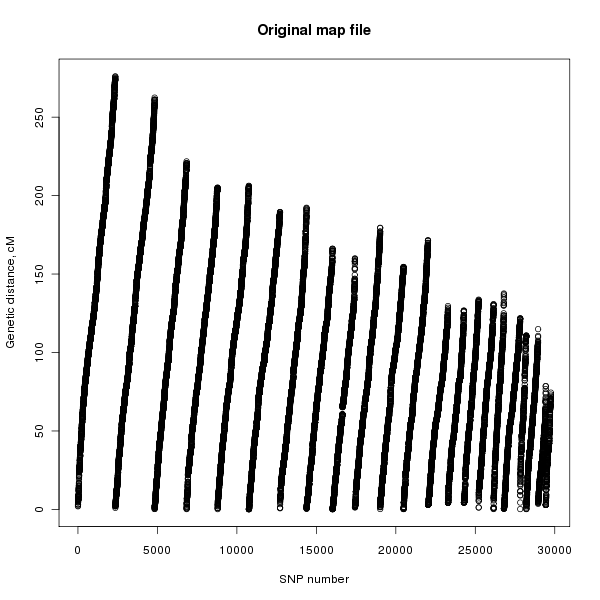
\includegraphics[width=200pt]{originalMap.png}}
\caption{Plot of the genetic distance against the SNP number for the original SNP file.}
\label{orig-fig}
\end{center}}
\end{figure}
}
{\begin{figure}[ht]
{\begin{center}
{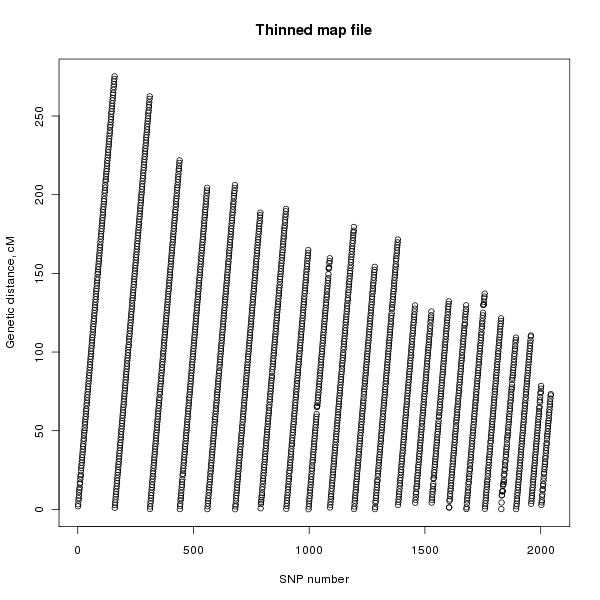
\includegraphics[width=200pt]{thinnedMap.png}}
\caption{Plot of the genetic distance against the SNP number for the thinned SNP file.}
\label{thin-fig}
\end{center}}
\end{figure}
}

{\bf Other Example Commands} 
\begin{enumerate}

\item {\bf Keep 2.6 SNPs per cM.} \vspace{0.35cm} \begin{lstlisting}

./mapthin -t 2.6 myfile.map mythinnedfile.map

\end{lstlisting} \vspace{0.35cm}
\item {\bf Keep 45.6\% of the SNPs in the map file.} \vspace{0.35cm} \begin{lstlisting}

./mapthin -p 45.6 myfile.map mythinnedfile.map

\end{lstlisting} \vspace{0.35cm}
\item {\bf Only output SNP names to the thinned map file.} \vspace{0.35cm} \begin{lstlisting}

./mapthin -n myfile.map mythinnedfile.map

\end{lstlisting} \vspace{0.35cm}
\item {\bf Keep 5.4 SNPs per $10^6$ base pair position of the SNPs in the map file.} \vspace{0.35cm} \begin{lstlisting}

./mapthin -b 5.4 myfile.map mythinnedfile.map

\end{lstlisting} \vspace{0.35cm}
\item {\bf Keep 23.7\% of the SNPs in the map file using base pair position instead of genetic distance.} \vspace{0.35cm} \begin{lstlisting}

./mapthin -b -p 23.7 myfile.map mythinnedfile.map

\end{lstlisting} \vspace{0.35cm}
\item {\bf Keep 4500 of the SNPs in the map file using base pair position instead of genetic distance.} \vspace{0.35cm} \begin{lstlisting}

./mapthin -b -s 4500 myfile.map mythinnedfile.map

\end{lstlisting} \vspace{0.35cm}\end{enumerate}
\end{document}